\documentclass[../thesis/thesis.tex]{subfiles}
\begin{document}

\chapter{Evaluation}
\label{chap:evaluation}

We believe it is possible to produce a VC investment screening system that is efficient, robust and powerful. In the previous chapter, we describe the development and structure of such a system. Our system is based around identifying startup companies that are likely to receive additional funding or a liquidity event (exit) in a given forecast window. This system can generate statistics and make recommendations that may assist VC firms to efficiently and effectively screen investment candidates. In this chapter, we evaluate models developed by our system against criteria of efficiency, robustness and predictive power. We discuss our findings more broadly and their implications for investors and future research into startup investment and performance.

In the previous chapter, we produced a classification pipeline which we optimised with respect to the robustness of its performance over time. In this chapter, we evaluate the performance of models produced by this pipeline against a held-out test dataset. This evaluation process is depicted in \ref{fig:evaluation:pipeline_evaluation}. We use the pipeline to fit a model to a dataset sliced from the master database. We apply this model to another feature vector from the master database and make predictions. We score these predictions against truth values derived from the held-out test database (collected in April 2017). This process is performed multiple times to evaluate the three primary criteria derived from our literature review: efficiency, robustness and predictive power. In this chapter, we evaluate our system against that criteria. The experiments are as follows: efficiency, the pipeline is fitted to datasets of various sample sizes; robustness, the pipeline is fitted to datasets from various time slices; and predictive power, the forecast window between the feature vector and outcome is varied.

Firstly, we evaluate efficiency by exploring the learning curves of our classification techniques and whether there is sufficient data to produce reliable statistics. We also epxlore the time profile of our system and whether it is reasonable for use in industry, and would be likely to reduce the time currently taken to perform similar analyses. Secondly, we evaluate robustness by evaluating our models against multiple reverse-engineered historical datasets and measuring their variance. Thirdly, we evaluate the system's predictive power across different forecast windows,  for startups at different stages of their development lifecycle, and for different potential target outcomes.

\begin{figure}[!htb]
    \centering
    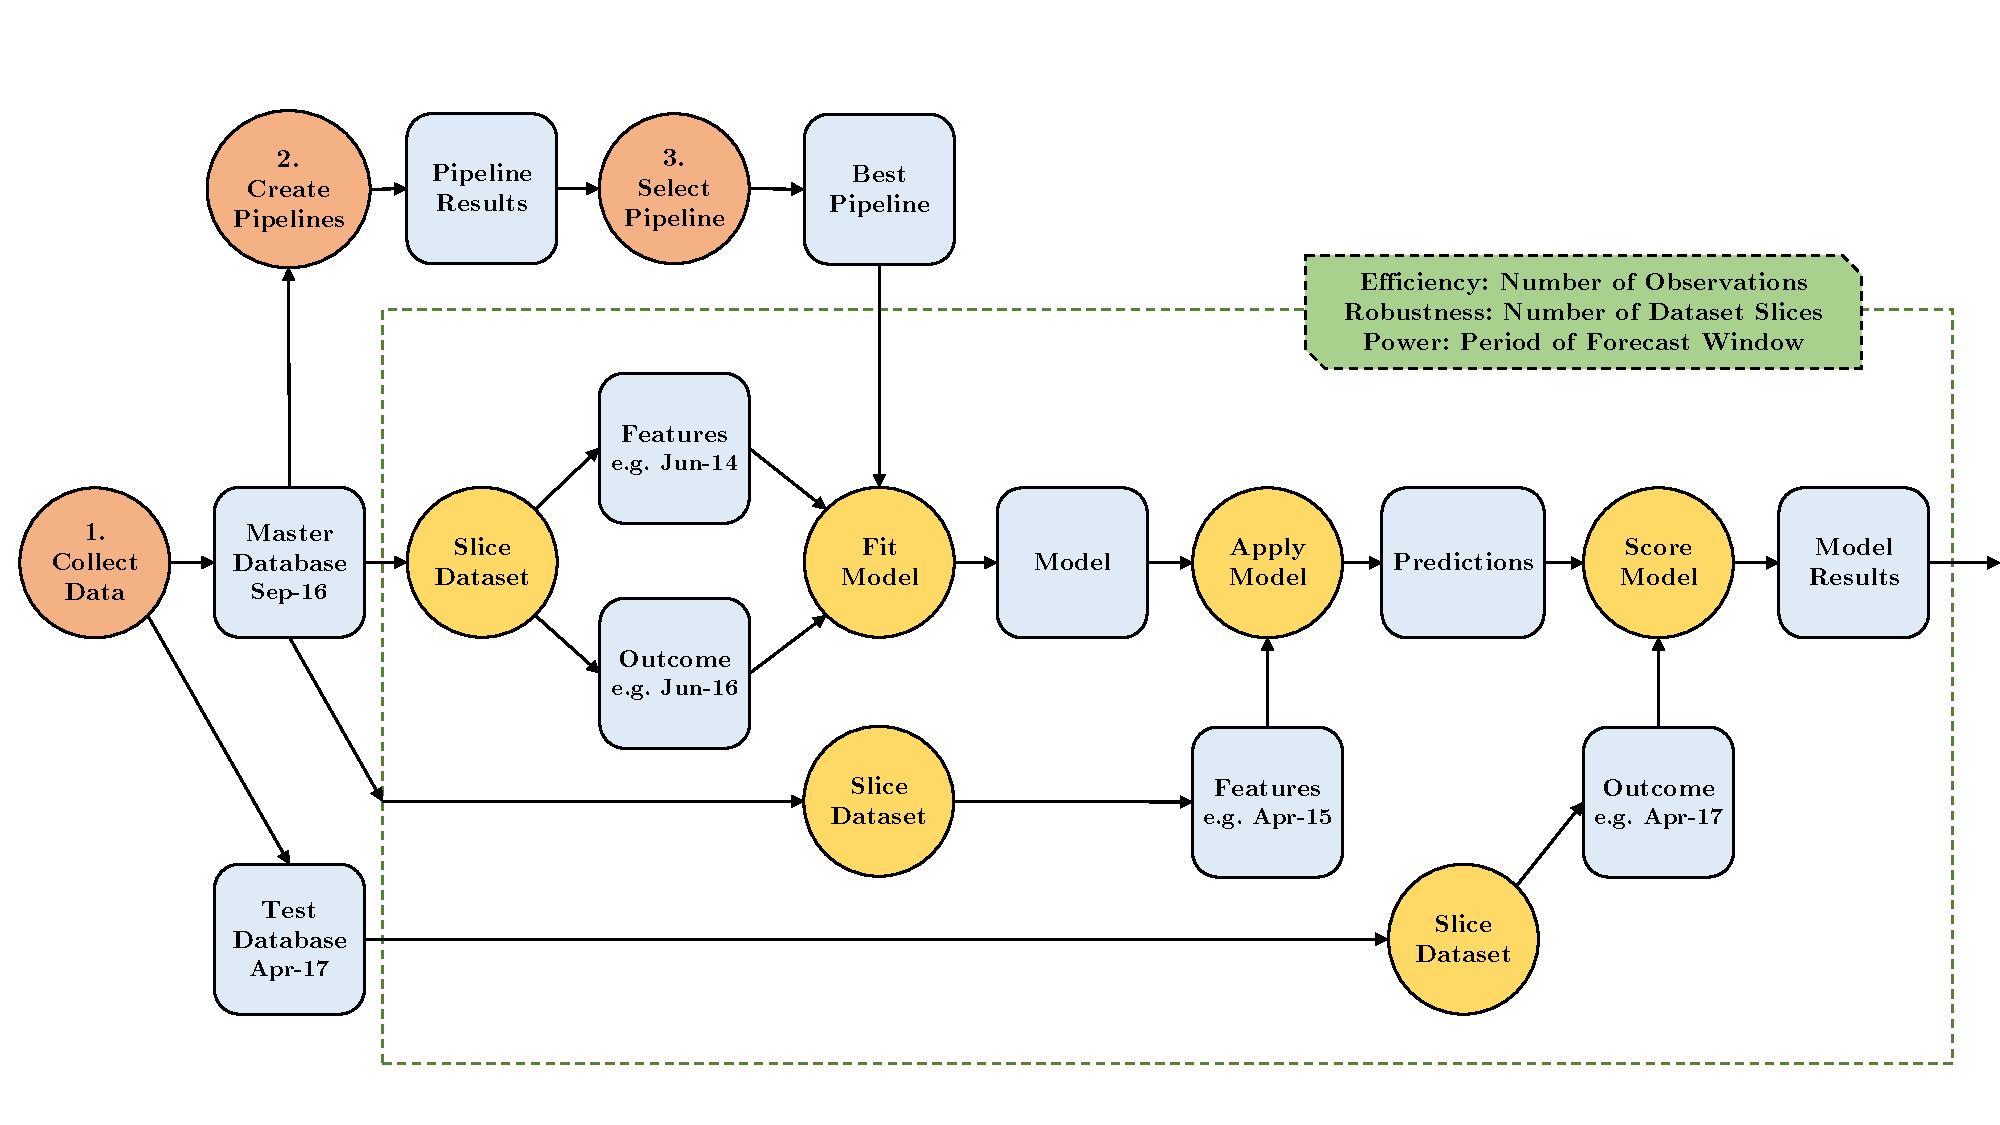
\includegraphics[width=\textwidth]{../figures/evaluation/pipeline_evaluation}
    \caption[Pipeline evaluation flowchart]{Pipeline evaluation overview.}
    \label{fig:evaluation:pipeline_evaluation}
\end{figure}

\section{Efficiency}

The gls\{vc} industry requires more efficient forms of \gls{vc} investment analysis, particularly in surfacing and screening. These processes are currently performed through referral, Google search, industry papers and manual search of startup databases. By its nature, our automated system should be more efficient than these methods. In this section, we assess how efficient our system is -- in terms of data consumed and time taken -- and look at whether we can further improve its efficiency.

\subsection{Dataset Size}

Learning curves show how the bias and variance of a classification technique varies with respect to the amount of training data available. We decided to investigate the learning curves for our classification pipeline to determine whether we could use smaller samples from our dataset to achieve similar predictive power and reduce our need for computational power and time taken. We applied 10-fold stratified cross-validation to split our dataset into 10 subsets of different sizes which we used to train the estimator and produce training and test scores for each subset size. The convergence or divergence of our training and cross-validation curves will imply whether our classification pipeline is over- or under-fitting our data for various sizes allowing us to select an optimal sample size. Figure~\ref{fig:evaluation:efficiency_learning_curve} shows the learning curves for forecast windows of 2-4 years, aggregated over multiple time slices. The maximum number of training examples is negatively related to the length of the forecast window because newer datasets have more examples. Visually, all three sub-figures are similar in nature. %TODO

\begin{figure}[!htb] %FUCKED UP - SHOULD CV ON FIT, NOT ON SCORE
    \centering
    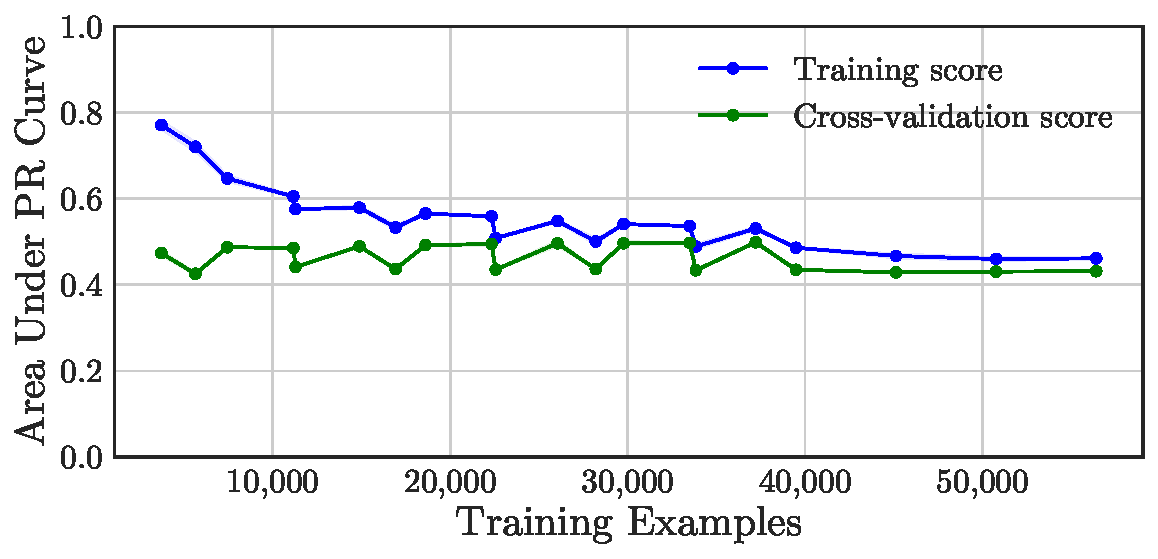
\includegraphics[width=\textwidth]{../figures/evaluation/efficiency_learning_curve}
    \caption[Learning curve]{}
    \label{fig:evaluation:efficiency_learning_curve}
\end{figure}

\subsection{Time Profile}

Unlike other forms of finance, like equity or derivatives trading, \gls{vc} operates on a much longer timeframe -- deals typically close over weeks, rather than minutes. This has two key disadvantages: \gls{vc} firms have higher management costs because they spend more time screening investments and startup founders waste precious time negotiating with investors when they could be building their businesses. Automated systems could significantly decrease the time taken to generate investment opportunities. We investigated the time profile of our system to determine whether it is practical for use in the \gls{vc} industry. The time profile of the system is shown in Figure~\ref{fig:evaulation:time_profile}. At the highest-level, the program takes approximately 46 hours to complete on a modern desktop PC. When we further break this time down by system component, it's clear that the vast majority of time (84.8\%) is taken up by the initial pipeline creation component. This time is due to the pipeline optimisation process - the model is fit and scored over 500 times on different classification algorithms and parameters. Scoring takes a particularly long time because, in this case, it also involves generating learning curves for reporting, which is another cross-validated process. However, when placed into production, this component could be run infrequently - perhaps once per year - to ensure that the pipelines being used are still optimally suited for the dataset. The next component of the system, selecting the most robust pipeline, could occur more frequently - perhaps once every month - and the final component of the pipeline, making up-to-date predictions, could be evaluated every time new data is fed into the system (perhaps once per day) because it only takes an hour.

\begin{table}[!htb]
    \centering
    \scalebox{0.9}{\newcommand{\sub}[1]{\hspace{1em}#1}

\begin{tabular}{lrrrrr} \toprule
Function & Cycle (s) & Cycles (N) & Time (s)   & Time (m) & Time (h) \\ \midrule
Generate Dataset (CV)             & 1,800 & 1 & 1,800 & 30 & 0.5 \\
\sub{Prepare Feature Dataset}     & 1,200 & 1 & 1,200 & 20 & 0.3 \\
\sub{Prepare Outcome Dataset}     & 180 & 1 & 180 & 3 & 0.1 \\
\sub{Merge Datasets}              & 360 & 1 & 360 & 6 & 0.1 \\
\sub{Finalise Dataset}            & 60 & 1 & 60 & 1 & 0.0 \\
Fit and Score Model\textsuperscript{1} & 265 & 525 & 139,125 & 2,319 & 38.6 \\
\sub{Fit Model}                   & 15 & 525 & 7,875 & 131 & 2.2 \\
\sub{Score Model}                 & 250 & 525 & 131,250 & 2,188 & 36.5 \\ \midrule
\multicolumn{3}{l}{Subtotal: Create Pipelines} & 140,925 & 2,349 & 39.1 \\ \midrule
Get Finalist Pipelines            & 5 & 1 & 5 & 0 & 0.0 \\
Generate Dataset (CV)             & 1,800 & 5 & 1,800 & 30 & 0.5 \\
Fit and Score Model\textsuperscript{2} & 265 & 75 & 19,875 & 331 & 5.5 \\
Select Best Pipeline              & 5 & 1 & 5 & 0 & 0.0 \\ \midrule
\multicolumn{3}{l}{Subtotal: Select Best Pipeline} & 21,685 & 361 & 6.0 \\ \midrule
Generate Dataset (Training)       & 1,800 & 1 & 1,800 & 30 & 0.5 \\
Generate Dataset (Test)           & 1,800 & 1 & 1,800 & 30 & 0.5 \\
Fit Model                         & 30 & 1 & 30 & 1 & 0.0 \\
Make Predictions                  & 5 & 1 & 5 & 0 & 0.0 \\ \midrule
\multicolumn{3}{l}{Subtotal: Fit and Make Predictions} & 3,635 & 61 & 1.0 \\ \midrule
\multicolumn{3}{l}{Total}        & 166,245 & 2,771 & 46.2 \\
\bottomrule \end{tabular}
}
    \caption[System time profile]{}
    \label{fig:evaluation:time_profile}
\end{table}

\section{Robustness}

It is critical that our system is robust in its performance with respect to time so investors can rely on its predictions based on historical models. This has been identified as a key barrier to the adoption of automated systems by the \gls{vc} industry \cite{stone2014}. CrunchBase provides created and last-updated timestamps for each record in their CSV-formatted dumps (and also in the JSON-formatted responses from their API). We took advantage of this to produce a system that reverse-engineers previous database states by filtering the current database by only records that were created by a given 'slice' date.

\subsection{Preliminary Analysis}

We performed preliminary testing of this technique by comparing a historical CrunchBase database collected in December 2013 with a slice from our primary dataset collected in September 2016, as shown in Table~\ref{fig:evaluation:2013_slice_comparison}. While there are some differences, particularly in the IPO counts, we consider this to be satisfactory variance considering the 3-year time difference (i.e. perhaps some companies have been since removed from the database). The key relations for the purposes of our system are Companies, Funding Rounds and People, all of which had minor differences considering the size of these datasets. Table~\ref{fig:evaluation:slice_counts_over_time} shows company counts by startup development stage from different dataset slices. We limited our experiments to dataset slices from 2012-onwards because prior to 2012 the datasets become too small to use to make predictions (particularly given the class imbalance).

\begin{figure}[!htb]
    \centering
    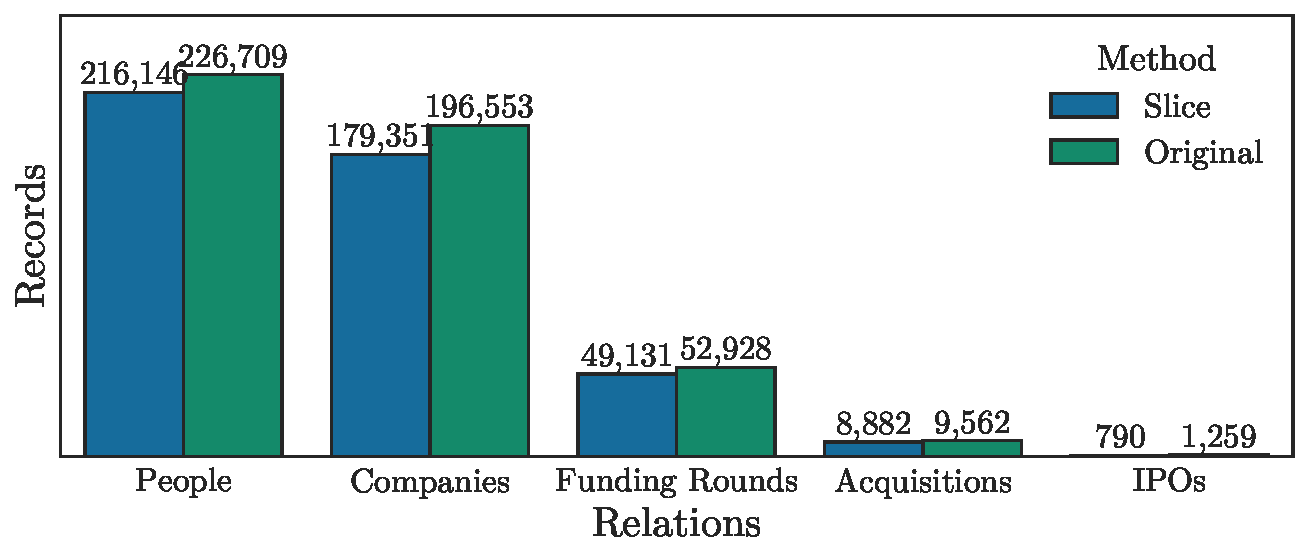
\includegraphics[width=\textwidth]{../figures/evaluation/2013_slice_comparison}
    \caption[Dataset slice compared with original dataset]{} %Needs caption
    \label{fig:evaluation:2013_slice_comparison}
\end{figure}

\begin{figure}[!htb]
    \centering
    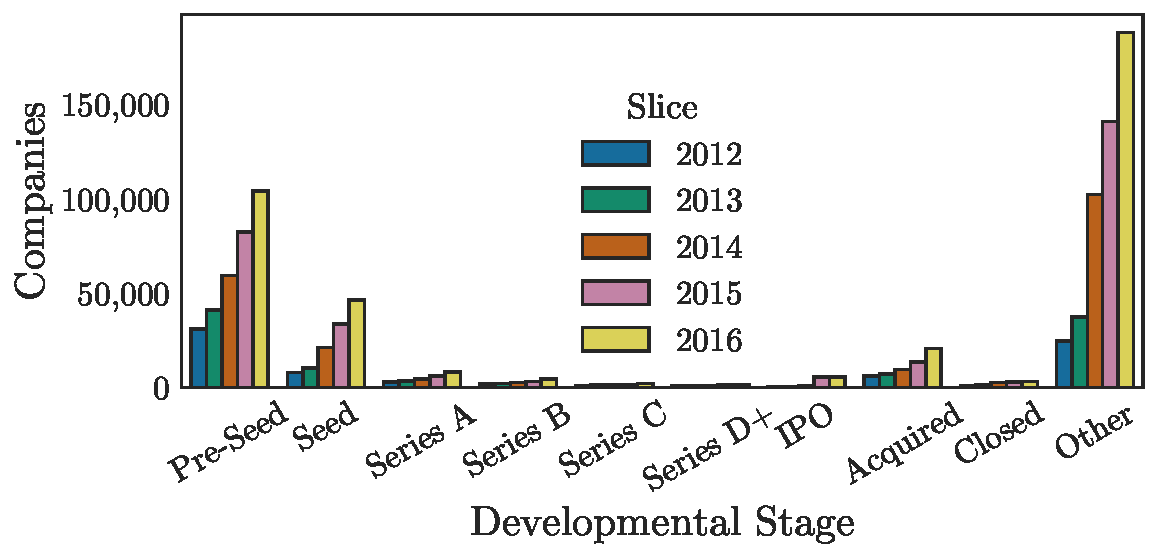
\includegraphics[width=\textwidth]{../figures/evaluation/slice_counts_over_time}
    \caption[Dataset counts over time]{} %Needs caption
    \label{fig:evaluation:slice_counts_over_time}
\end{figure}

\subsection{Dataset Slices}

We fit our model to three datasets created from our training database from each year of 2012-2014 (i.e. features|outcome: 2012|2014, 2013|2015, 2014|2016), and evaluated the model for forecast windows of 2 years, against a dataset created from our test database (i.e. 2015|2017). We expect that if the factors that predict startup investment success through time are consistent, we would observe little difference between the performance and characteristics of these models. Figure~\ref{fig:evaluation:pr_curve_slice} shows the characteristics of the Precision-Recall curves for each model. There is very little difference in the characteristics of each curve. We observe slightly higher precision for low recall values for the 2014 dataset, <WHY?>. Overall, the area under each curve is within the margin of error. Figure~\ref{fig:evaluation:clf_report_slice} shows the classification report for each model. The F1-Scores (Positive Class) are identical across the models, at 0.32. Finally, we explore the feature weights for each model in Figure~\ref{fig:evaluation:feature_groups_slice}. While there are some slight differences, the general trend is very similar across all models. All of these results suggest that our system generates models that are robust with respect to time.

\begin{figure}[!htb] %Labels might be reversed, figure too big
    \centering
    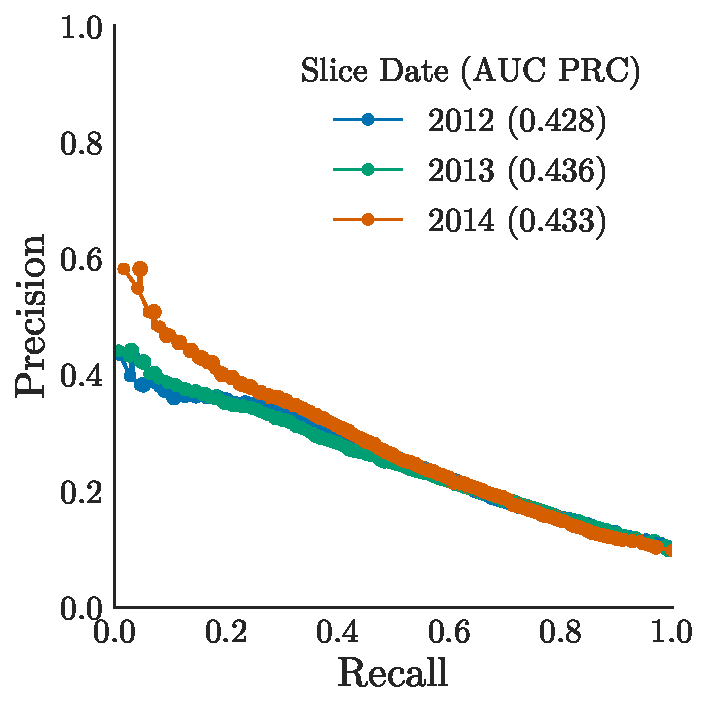
\includegraphics[width=\textwidth]{../figures/evaluation/pr_curve_slice}
    \caption[PR Curves by slice date]{} %Needs caption
    \label{fig:evaluation:pr_curve_slice}
\end{figure}

\begin{table}[!htb]
    \centering
    \scalebox{0.9}{\begin{tabular}{llrrrrrr} \toprule
\multicolumn{2}{l}{Slice Date} & N & (\%)    & Accuracy & Precision   & Recall & F1-Score \\ \midrule
2012 & Outcome=0 & 106,583 & (90.2\%) & - & 0.95 & 0.77 & 0.85 \\
     & Outcome=1 & 11,538 & (9.8\%) & - & 0.22 & 0.59 & 0.32 \\
     & Avg/Total & 118,121 & - & 0.76 & 0.88 & 0.76 & 0.80 \\
2013 & Outcome=0 & 106,489 & (90.2\%) & - & 0.95 & 0.75 & 0.84 \\
     & Outcome=1 & 11,535 & (9.8\%) & - & 0.21 & 0.62 & 0.32 \\
     & Avg/Total & 118,024 & - & 0.74 & 0.88 & 0.74 & 0.79 \\
2014 & Outcome=0 & 106,583 & (90.2\%) & - & 0.95 & 0.76 & 0.84 \\
     & Outcome=1 & 11,538 & (9.8\%) & - & 0.21 & 0.61 & 0.32 \\
     & Avg/Total & 118,121 & - & 0.74 & 0.88 & 0.74 & 0.79 \\
\bottomrule \end{tabular}
}
    \caption[Classification report by slice date]{} %Needs caption
    \label{fig:evaluation:clf_report_slice}
\end{table}

\begin{figure}[!htb]
    \centering
    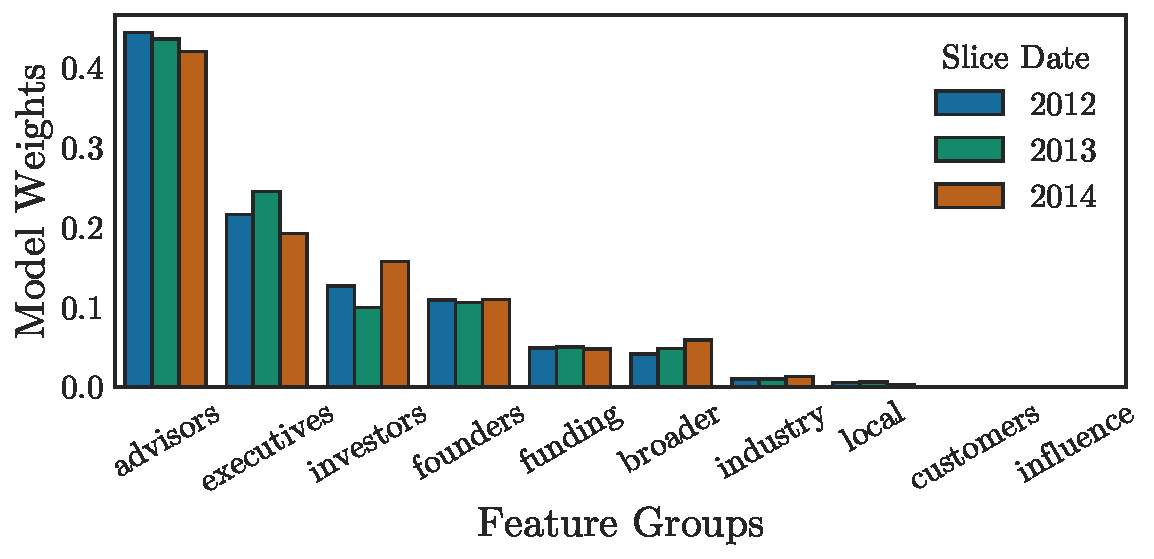
\includegraphics[width=\textwidth]{../figures/evaluation/feature_groups_slice}
    \caption[Grouped feature weights by slice date]{} %Needs caption
    \label{fig:evaluation:feature_groups_slice}
\end{figure}

\section{Predictive Power}


\subsection{Preliminary Analysis}

Finally, we test our system's predictive power for making forecasts of different time periods. We use the same system of reverse-engineering time slices that we used in our previous experiment to robustness, but this time we vary the time difference between the slice that provides our features and the slice that provides our outcome.
We performed preliminary testing by combining pair-wise datasets of each year from 2012-2016 inclusive and exploring the proportion of companies that raised additional funding or exited (for brevity, we will call this ``investment success''. Figure~\ref{fig:evaluation:outcome_forecast_window} shows how investment success varies with respect to the forecast window (time between the observed features and the measured outcome). Intuitively, we see a positive relationship between length of forecast window and investment success. In particular, very few companies appear to have investment success over a period of less than 2 years so we will focus our experimentation on forecast windows of 2--4 years.

\begin{figure}[!htb] %Split by target outcome
    \centering
    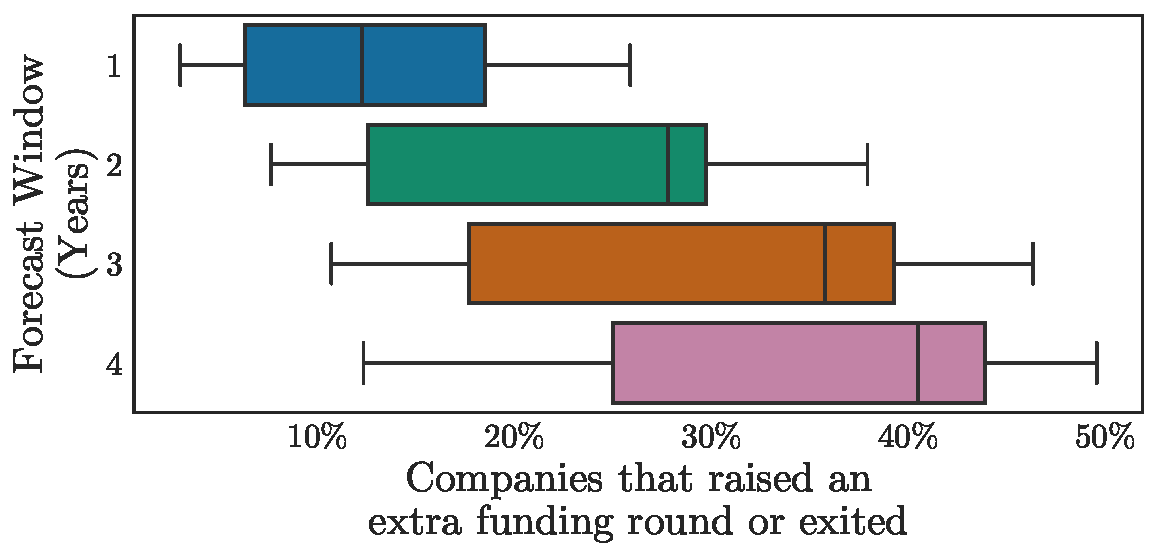
\includegraphics[width=\textwidth]{../figures/evaluation/outcome_forecast_window}
    \caption[Investment success by forecast window]{} 
    \label{fig:evaluation:outcome_forecast_window}
\end{figure}

We also looked at how investment success varies with respect to development stage, shown in Figure~\ref{fig:evaluation:outcome_stage}. We see a broad positive relationship between developmental stage and likelihood of investment success, which we would expect as at each stage there is higher market traction and scrutiny from investors. One exception is for companies at Series D+ stage, but this may reflect that these companies are aiming for an exit which likely takes longer than seeking additional funding rounds and so is less well shown in our dataset (which caps out at a forecast window of 4 years). The variance between the different developmental stages suggests that in our experimentation we should investigate how our system predicts each stage independently, as well as in aggregate.

\begin{figure}[!htb]  %Split by target outcome
    \centering
    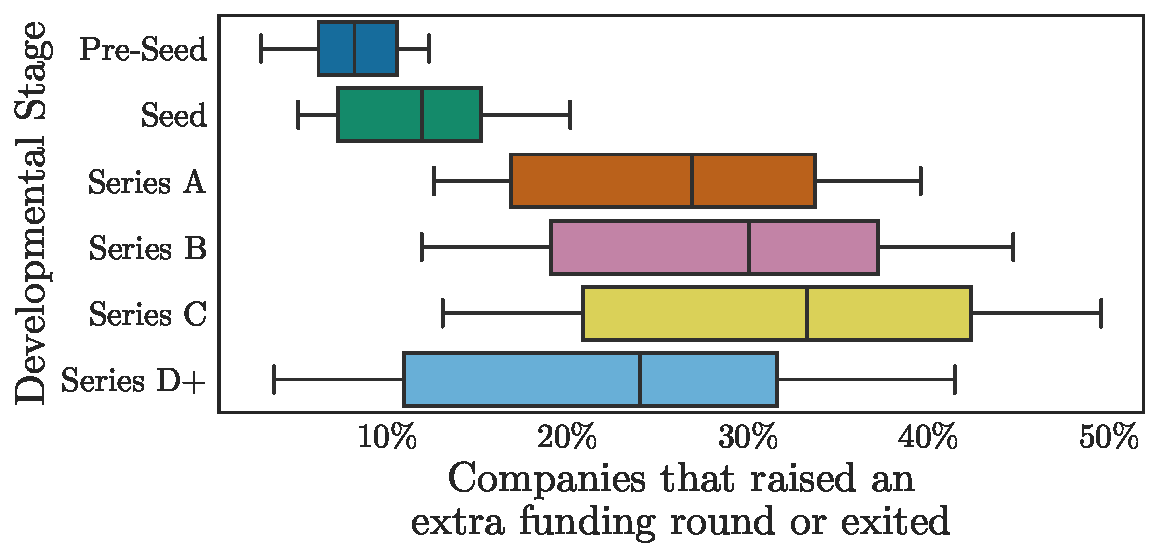
\includegraphics[width=\textwidth]{../figures/evaluation/outcome_stage}
    \caption[Investment success by developmental stage]{}
    \label{fig:evaluation:outcome_stage}
\end{figure}

\subsection{Forecast Windows}

%TODO

\begin{figure}[!htb]
    \centering
    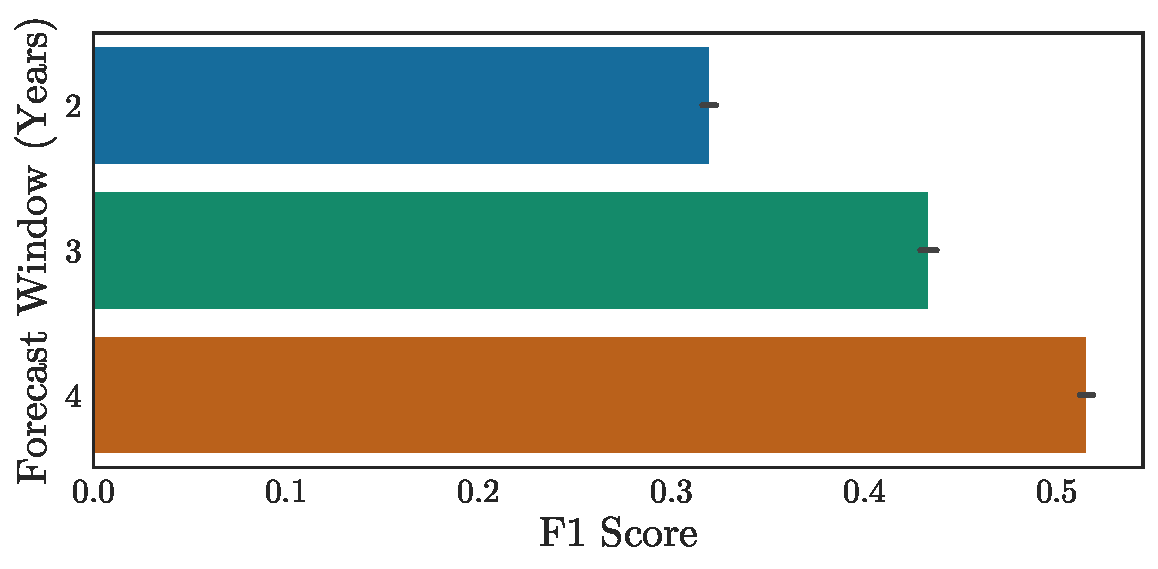
\includegraphics[width=\textwidth]{../figures/evaluation/predictive_window}
    \caption[F1 Scores by forecast window]{}
    \label{fig:evaluation:f1_predictive_window}
\end{figure}

\begin{table}[!htb]
    \centering
    \scalebox{0.9}{\begin{tabular}{llrrrrr} \toprule
Forecast Window  & & N (\%)    & Accuracy & Precision   & Recall & F1-Score \\ \midrule
2 Years & Outcome=0 & 319,655 (90.2\%) & - & 0.95 & 0.76 & 0.84 \\
        & Outcome=1 & 34,611 (9.8\%) & - & 0.22 & 0.61 & 0.32 \\
        & Avg/Total & 354,266 & 0.75 & 0.88 & 0.75 & 0.79 \\
3 Years & Outcome=0 & 216,816 (85.6\%) & - & 0.93 & 0.77 & 0.84 \\
        & Outcome=1 & 36,602 (14.4\%) & - & 0.32 & 0.66 & 0.43 \\
        & Avg/Total & 253,418 & 0.75 & 0.84 & 0.75 & 0.78 \\
4 Years & Outcome=0 & 137,217 (81.9\%) & - & 0.91 & 0.81 & 0.86 \\
        & Outcome=1 & 30,255 (19.1\%) & - & 0.43 & 0.65 & 0.52 \\
        & Avg/Total & 167,472 & 0.78 & 0.82 & 0.78 & 0.80 \\
\bottomrule \end{tabular}
}
    \caption[Classification report by forecast window]{}
    \label{fig:evaluation:clf_report_window}
\end{table}

\begin{figure}[!htb]
    \centering
    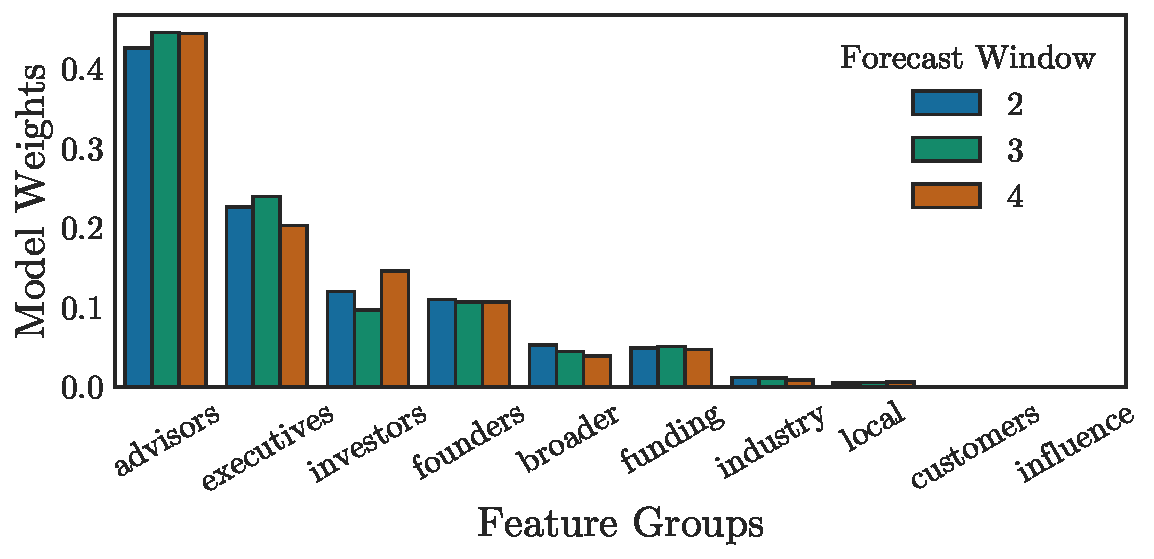
\includegraphics[width=\textwidth]{../figures/evaluation/feature_groups_window}
    \caption[Grouped feature weights by forecast window]{}
    \label{fig:evaluation:feature_groups_window}
\end{figure}

\subsection{Development Stage}

%TODO

\begin{figure}[!htb]
    \centering
    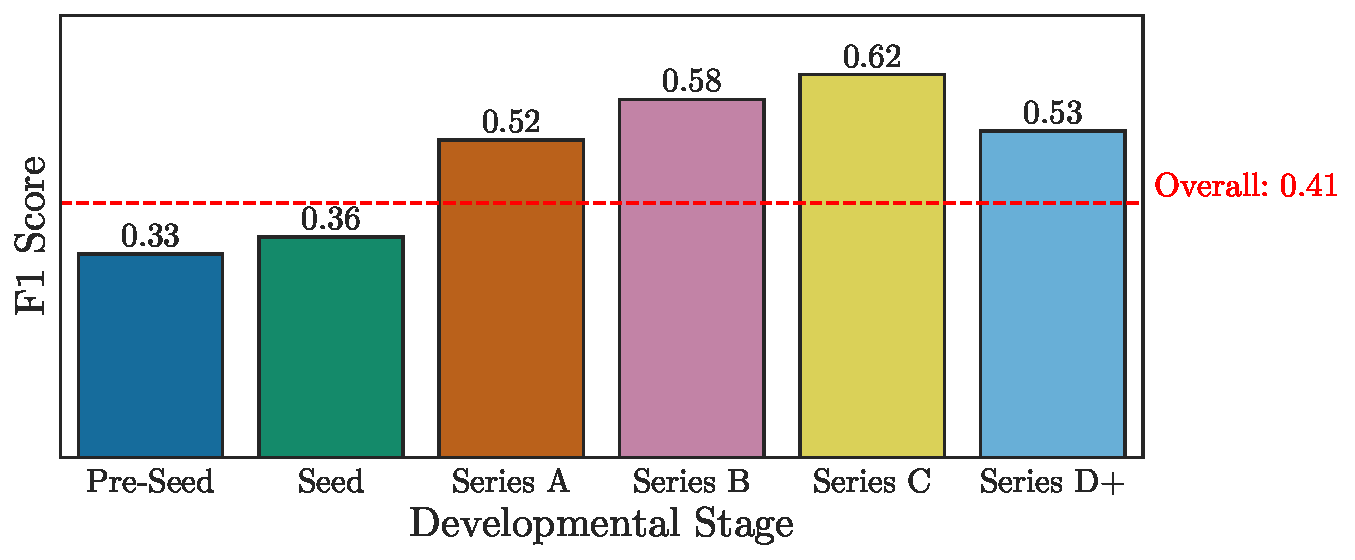
\includegraphics[width=\textwidth]{../figures/evaluation/predictive_stage}
    \caption[F1 Scores by developmental stage]{}
    \label{fig:evaluation:f1_predictive_stage}
\end{figure}

\begin{table}[!htb]
    \centering
    \scalebox{0.9}{\begin{tabular}{llrrrrrr} \toprule
\multicolumn{2}{l}{Stage} & N & (\%)    & Accuracy & Precision   & Recall & F1-Score \\ \midrule
Pre-Seed     & Outcome=0 & 491,154 & (90.4\%) & - & 0.94 & 0.88 & 0.91 \\
             & Outcome=1 & 51,862 & (9.6\%) & - & 0.27 & 0.42 & 0.33 \\
             & Avg/Total & 543,016 & - & 0.84 & 0.87 & 0.84 & 0.85 \\
Seed         & Outcome=0 & 136,586 & (85.7\%) & - & 0.93 & 0.60 & 0.73 \\
             & Outcome=1 & 22,872 & (14.3\%) & - & 0.24 & 0.74 & 0.36 \\
             & Avg/Total & 159,458 & - & 0.62 & 0.83 & 0.62 & 0.68 \\
Series A     & Outcome=0 & 23,861 & (67.6\%) & - & 0.87 & 0.18 & 0.30 \\
             & Outcome=1 & 11,427 & (32.4\%) & - & 0.36 & 0.94 & 0.52 \\
             & Avg/Total & 35,288 & - & 0.43 & 0.71 & 0.43 & 0.37 \\
Series B     & Outcome=0 & 12,116 & (59.3\%) & - & 0.84 & 0.04 & 0.07 \\
             & Outcome=1 & 8,314 & (40.7\%) & - & 0.41 & 0.99 & 0.58 \\
             & Avg/Total & 20,430 & - & 0.43 & 0.66 & 0.43 & 0.28 \\
Series C     & Outcome=0 & 5,555 & (55.2\%) & - & 0.82 & 0.03 & 0.07 \\
             & Outcome=1 & 4,516 & (44.8\%) & - & 0.45 & 0.99 & 0.62 \\
             & Avg/Total & 10,071 & - & 0.46 & 0.66 & 0.46 & 0.32 \\
Series D+    & Outcome=0 & 4,416 & (64.1\%) & - & 0.89 & 0.02 & 0.03 \\
             & Outcome=1 & 2,477 & (35.9\%) & - & 0.36 & 1.00 & 0.53 \\
             & Avg/Total & 6,893 & - & 0.37 & 0.70 & 0.37 & 0.21 \\
\bottomrule \end{tabular}
}
    \caption[Classification report by developmental stage]{}
    \label{fig:evaluation:clf_report_stage}
\end{table}

\begin{figure}[!htb]
    \centering
    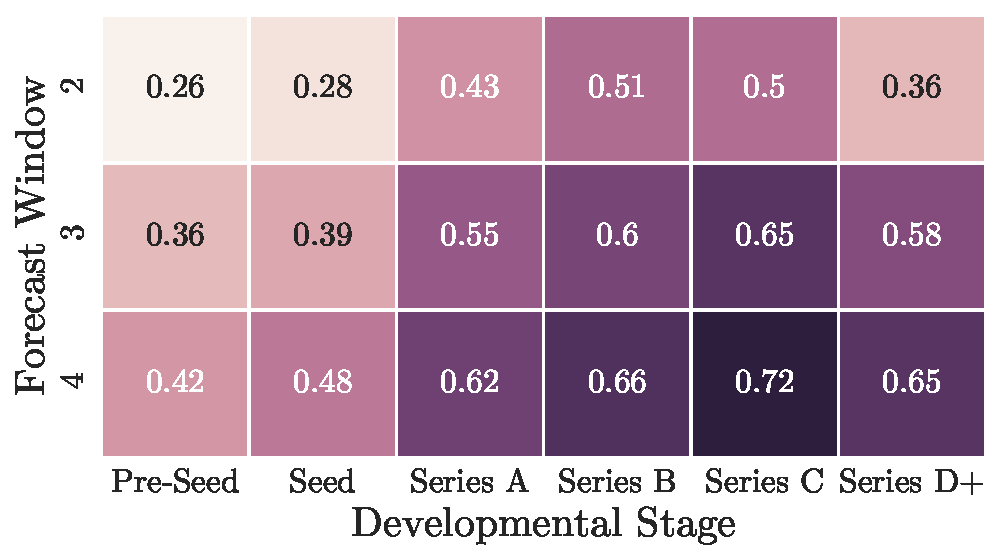
\includegraphics[width=\textwidth]{../figures/evaluation/predictive_heatmap}
    \caption[F1 Scores by developmental stage and forecast window]{}
    \label{fig:evaluation:f1_predictive_heatmap}
\end{figure}

\begin{figure}[!htb]
    \centering
    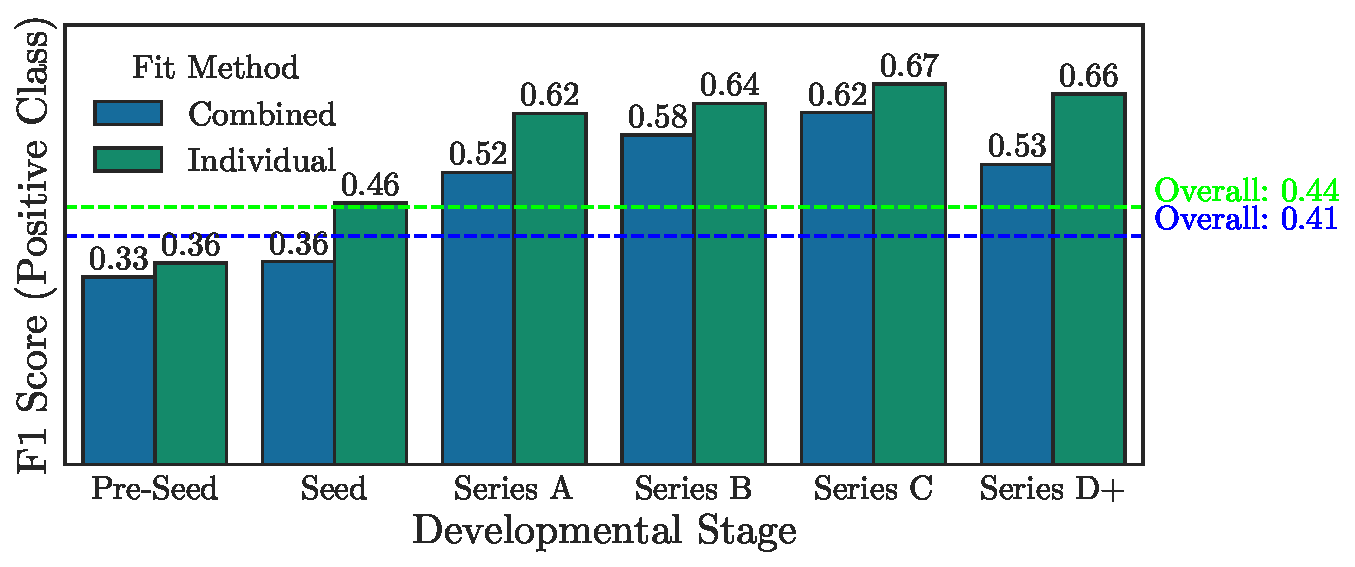
\includegraphics[width=\textwidth]{../figures/evaluation/f1_individual_overall}
    \caption[F1 Scores by moodel fit method]{}
    \label{fig:evaluation:f1_individual_overall}
\end{figure}

\begin{figure}[!htb]
    \centering
    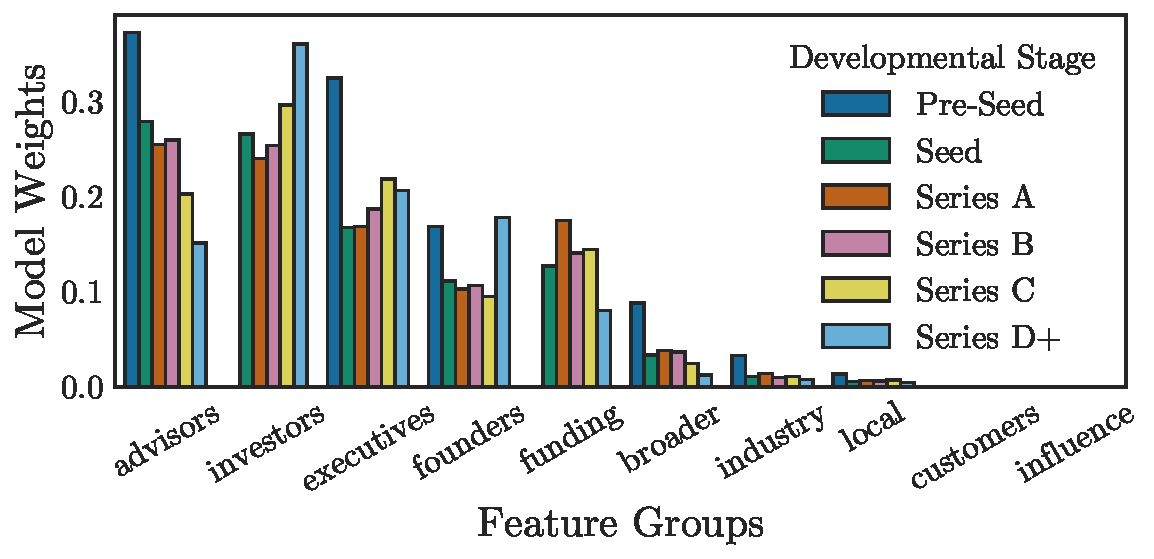
\includegraphics[width=\textwidth]{../figures/evaluation/feature_groups_stage}
    \caption[Grouped feature weights by developmental stage]{}
    \label{fig:evaluation:feature_groups_stage}
\end{figure}

\subsection{Target Outcomes}

%TODO

\begin{figure}[!htb] %WIP
    \centering
    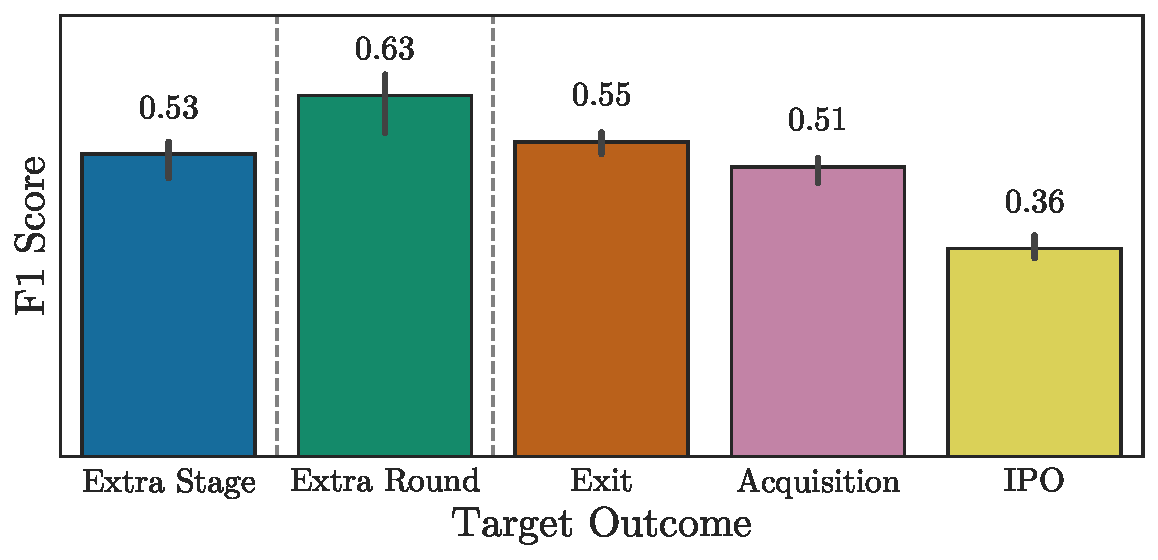
\includegraphics[width=\textwidth]{../figures/evaluation/f1_predictive_outcome}
    \caption[F1 Scores by target outcome]{}
    \label{fig:evaluation:f1_predictive_outcome}
\end{figure}

\begin{table}[!htb] %WIP
    \centering
    \scalebox{0.9}{\begin{tabular}{llrrrrrr} \toprule
\multicolumn{2}{l}{Target Outcome} & N       & \%   & Accuracy  & Precision  & Recall  & F1   \\ \midrule
Extra Stage & Positive & 30,279  & 18.0 & -    & 0.50 & 0.61 & 0.55 \\
            & Negative & 137,646 & 82.0 & -    & 0.91 & 0.86 & 0.89 \\
            & Avg/Total & 167,925 & -    & 0.82 & 0.84 & 0.82 & 0.83 \\ \midrule
Extra Round & Positive & 21,588  & 12.9 & -    & 0.34 & 0.61 & 0.44 \\
            & Negative & 146,337 & 87.1 & -    & 0.93 & 0.83 & 0.88 \\
            & Avg/Total & 167,925 & -    & 0.80 & 0.86 & 0.80 & 0.82 \\ \midrule
Exit        & Positive & 12,372  & 17.4 & -    & 0.46 & 0.70 & 0.56 \\
            & Negative & 155,553 & 92.6 & -    & 0.97 & 0.94 & 0.96 \\
            & Avg/Total & 167,925 & -    & 0.92 & 0.94 & 0.92 & 0.93 \\ \midrule
Acquisition & Positive & 10,566  & 16.3 & -    & 0.40 & 0.71 & 0.51 \\
            & Negative & 157,359 & 93.7 & -    & 0.98 & 0.93 & 0.95 \\
            & Avg/Total & 167,925 & -    & 0.91 & 0.94 & 0.91 & 0.93 \\ \midrule
IPO         & Positive & 2,052   & 1.2  & -    & 0.28 & 0.57 & 0.37 \\
            & Negative & 165,873 & 98.8 & -    & 0.99 & 0.98 & 0.99 \\
            & Avg/Total & 167,925 & -    & 0.98 & 0.99 & 0.98 & 0.98 \\
\bottomrule \end{tabular}

% @ 4 Years
}
    \caption[Classification report by target outcome]{}
    \label{fig:evaluation:clf_report_outcome}
\end{table}

\begin{figure}[!htb] %WIP
    \centering
    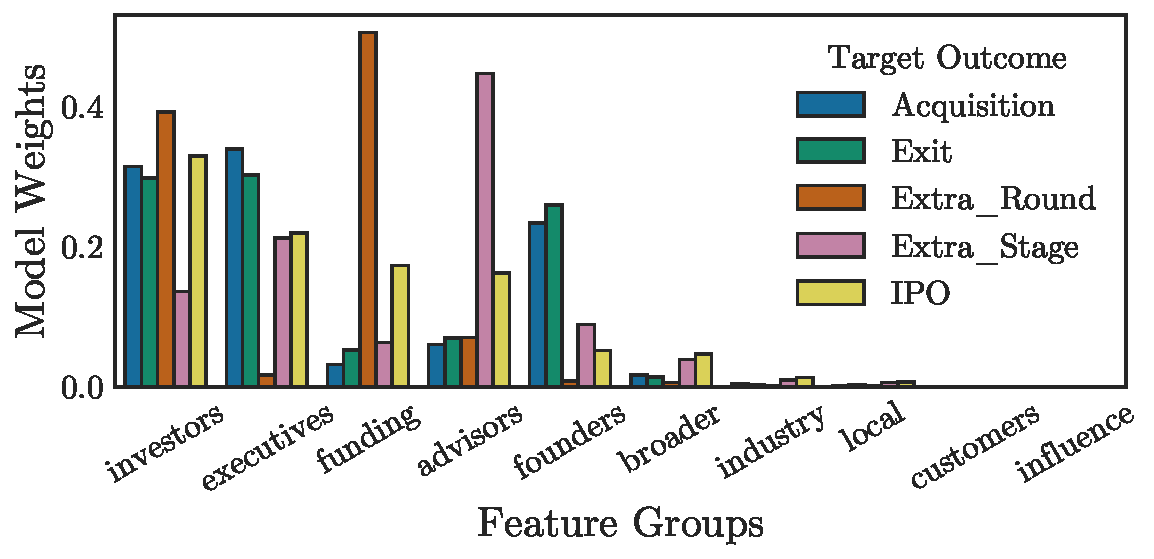
\includegraphics[width=\textwidth]{../figures/evaluation/feature_groups_outcome}
    \caption[Grouped feature weights by target outcome]{}
    \label{fig:evaluation:feature_groups_outcome}
\end{figure}

\begin{table}[!htb]
    \centering
    \scalebox{0.9}{\begin{tabular}{lrrrrrrrrr} \toprule
& \multicolumn{3}{c}{Company} \\
Feature                 & Company1  & Company2  & Company3  \\ \midrule
Feature1                & Count1    & Count2    & Count3    \\
Feature2                & Count1    & Count2    & Count3    \\
Feature3                & Count1    & Count2    & Count3    \\ \midrule
P(Outcome=1 | X)        & Count1    & Count2    & Count3    \\
Predicted Outcome       & Count1    & Count2    & Count3    \\
Actual Outcome          & Count1    & Count2    & Count3    \\
Correct Prediction      & Count1    & Count2    & Count3    \\
\bottomrule \end{tabular}
}
    \caption[Example company profiles and their predictions]{}
    \label{fig:evaluation:example_predictions}
\end{table}

 \ifcsdef{mainfile}{}{\printbibliography}
\end{document}
